\documentclass[12pt]{extarticle}

\setlength{\headheight}{16pt} % ??? we do what fancyhdr tells us to do  

\title{Physics 2}
\author{Giacomo Ellero}
\date{a.y. 2024/2025}

\usepackage[arrowdel]{physics}
\usepackage{siunitx}
\usepackage{preamble}
\usepackage{preamble_svg}

% \renewcommand{\vec}[1]{\uvec{#1}}

\begin{document}

\firstpage

\section{Mathematical tools}

\subsection{Scalar and vector fields}

\begin{definition}{Scalar field}{scalar-field}
    A scalar field is a function of type $f:\R^d \to \R$.
\end{definition}

Some examples of scalar fields are temperature or pressure.

\begin{definition}{Level curve of a scalar field}{level-curve-scalar}
    Let $f$ be a scalar field and $k \in \R$ constant.
    Then a level curve of $f$ at $k$ is the set
    \begin{equation}
        \left\{ \vec x \in \R^d : f(\vec x) = k  \right\}
    \end{equation}
\end{definition}


\begin{definition}{Vector field}{vector-field}
    A vector field is a function of type $\vec v: \R^d \to \R^d$.
\end{definition}

Some examples of vector fields are gravitational fields or the velocity field of fluids.

We will always work with \say{well behaved} fields: this means the functions are \say{almost always infinite} (of class $C^\infty$ with only some points as exceptions).

\begin{example}{Vector field}{vec-field}
    Let $\vec v(x, y, z) = x \hat x + y \hat y + z \hat z$.

    \begin{figure}[H]
        \centering
        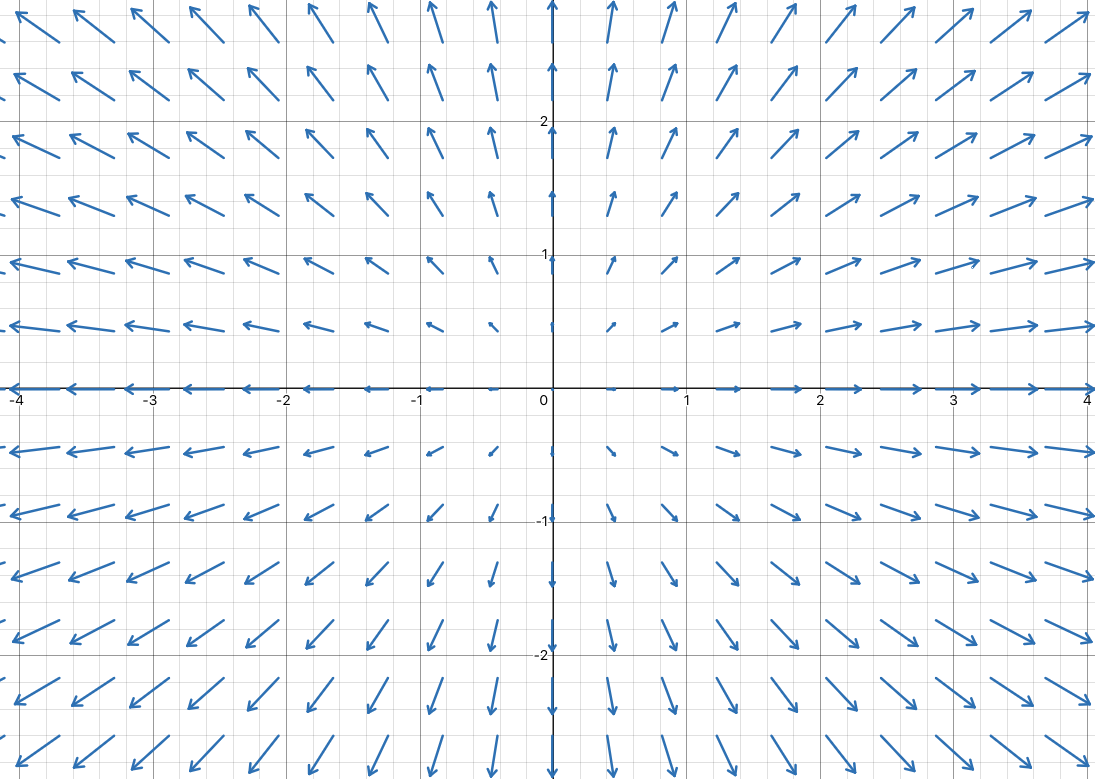
\includegraphics[height=0.4\textwidth]{assets/physics-2/vector-field-example.png}
        \caption{The arrow representation of $\vec v$ when $z = 0$.}
        \label{fig:field_source_0}
    \end{figure}
\end{example}

Some vector fields have \say{special points} where there are an infinite number of field lines going through it:
\begin{itemize}
    \item If all the lines go into that point we call such point \textbf{source} (the point $(0,0,0)$ is a source for \Cref{ex:vec-field});
    \item If all the lines go out of that point we call such point \textbf{sink} (use the field $\vec v(x, y, z) = -x \hat x - y \hat y - z \hat z$ as an example).
\end{itemize}
It is possible for some vector fields to have no sources or sinks. Some patterns that can arise are \textit{loops} or \textit{straight lines}.

\subsection{Operations over fields}

\begin{definition}{Gradient of a scalar field}{gradient-scalar}
    We define the gradient as
    \begin{equation}
        \grad f = \pdv{f}{x} \hat{x} + \pdv{f}{y} \hat{y} + \pdv{f}{z} \hat{z}
    \end{equation}

    We can also define the differential of a field as follows (where $\dd{l} = \dd{x} \hat{x} + \dd{y} \hat{y} + \dd{z} \hat{z} $):
    \begin{equation}
        \dd{f} = \pdv{f}{x} \dd{x} + \pdv{f}{y} \dd{y} + \pdv{f}{z} \dd{z} = \grad f \cdot \dd{\vec l}
    \end{equation}
\end{definition}

The gradient of a field is somewhat the equivalent of the derivative for 1D functions.

\begin{proposition}{Properties of the gradient}{props-gradient}
    \begin{enumerate}[label=\roman*.]
        \item $\grad f$ is orthogonal to the level curves;
        \item $\grad f$ points in the direction of the steepest ascent;
    \end{enumerate}
\end{proposition}

\begin{definition}{Directional derivative}{directional-derivative}
    The directional derivative is the slope of the field in the direction $\vec l$.
    \begin{equation}
        \dv{f}{l} = \grad \cdot \dd{\vec l}
    \end{equation}
\end{definition}

\begin{definition}{Gradient (nabla) operator}{nabla-operator}
    We define the nabla operator as
    \begin{equation}
        \grad = \pdv{}{x} \hat{x} + \pdv{}{y} \hat{y} + \pdv{}{z} \hat{z}
    \end{equation}
\end{definition}

This operator is particularly useful because we can treat it basically like a vector: when we multiply the $\grad$ with a vector field $f$ we get the gradient field of $f$.

\begin{definition}{Divergence}{divergence}
    Let $\vec v$. Then
    \begin{align}
        \div \vec v & = \left( \pdv{}{x} \hat{x} + \pdv{}{y} \hat{y} + \pdv{}{z} \hat{z} \right) \cdot \left( v_x \hat x + v_y \hat y + v_z \hat z\right) \\
                    & = \pdv{v_x}{x} + \pdv{v_y}{y} + \pdv{v_z}{z}
    \end{align}
\end{definition}

The intuition behind divergence is to measure how much a field \say{spreads out} from the point where it is measured.

\begin{example}{}{}
    Take $\vec v$ as in \Cref{fig:field_source_0}. Then
    \begin{equation}
        \div \vec v = \pdv{x}{x} + \pdv{y}{y} + \pdv{z}{z} = 3
    \end{equation}

    We have that the divergence for this field is always positive therefore the arrows always go further away from each other.
\end{example}

\begin{example}{Solenoidal field}{solenoidal-field}
    Let $\vec v = \hat z$. We have $\div \vec v = 0$.

    Fields with zero divergence are called solenoidals.
\end{example}

\begin{definition}{Curl}{curl}
    Let $\vec v$ be a vector field. Then
    \begin{equation}
        \curl \vec f = \det\begin{vmatrix}
            \hat x    & \hat y    & \hat z    \\
            \pdv{}{x} & \pdv{}{y} & \pdv{}{z} \\
            v_x       & v_y       & v_z
        \end{vmatrix}
    \end{equation}
\end{definition}

The intuition behind curl is to measure how much a vector field rotates or spins around the point where we compute it.

\begin{proposition}{Linearity}{linearity-of-grad}
    $\grad(\mathord{\cdot})$, $\div(\mathord{\cdot})$, and $\curl(\mathord{\cdot})$ are linear operators.
\end{proposition}

\begin{proposition}{Leibniz rule}{leibniz-rule}
    \begin{equation}
        \grad{fg} = (\grad f)g + f (\grad g)
    \end{equation}
\end{proposition}

\subsubsection{Higher order derivatives}
\label{sec:higher-order-derivatives}

\begin{enumerate}
    \item \textit{Divergence of gradient}
          (also called \textit{laplacian}):

          \begin{align}
              \div (\grad \vec f) & = \left( \pdv{}{x} \hat{x} + \pdv{}{y} \hat{y} + \pdv{}{z} \hat{z} \right) \cdot \left( \pdv{f}{x} \hat{x} + \pdv{f}{y} \hat{y} + \pdv{f}{z} \hat{z} \right) \\
                                  & = \pdv[2]{f}{x} + \pdv[2]{f}{y} + \pdv[2]{f}{z} = \grad^2(f)
          \end{align}

    \item \textit{Curl of gradient}: $\curl(\grad f) = 0$ (Schwartz theorem holds).
    \item \textit{Gradient of divergence}: $\grad (\div \vec V)$ is usually not useful.
    \item \textit{Divergence of curl}: $\div (\curl \vec v) = 0$
    \item \textit{Curl of curl}: (not so frequent)
          \begin{equation}
              \curl (\curl \vec f) = \grad (\div \vec v) - \grad^2(\vec v)
          \end{equation}
          where $\grad^2(\vec v) = (\grad^2 v_x \hat x + \grad^2 v_y \hat y + \grad^2 v_z \hat z)$ is called the laplacian vector operator.
\end{enumerate}

\subsection{Integrals}

\subsubsection{Line integrals}

\begin{definition}{Line integral}{line-integral}
    Let $f$ be a scalar field and $\vec v$ a vector field.
    \begin{enumerate}
        \item $\int_C f \dd{s}$
        \item $\int_C \vec v \dd{\vec l}$
    \end{enumerate}
    where $\dd{\vec l}$ is tangent to $C$ at every point.
\end{definition}

Note that if $C$ is closed we will write $\oint$ instead of $\int$.

Moreover, some fields $\vec v$ are such that $\int_C \vec v \dd{\vec l}$ does not depend on $C$ but only on its endpoints.
These are called \textbf{conservative fields}.

\subsubsection{Surface integral}

Let a vector field $\vec v$ and an open surface $S$.
We define $\dd{\vec S}$ the infinitesimal area oriented normal to $S$: $\dd{\vec S} = \dd{S} \vec n$.

Then define the \textit{infinitesimal flux} over $S$ as
\begin{equation}
    \dd{\Phi_S(\vec v)} = \vec v \cdot \dd{\vec S}
\end{equation}

\begin{definition}{Flux}{flux}
    The flux of $\vec v$ over $S$ is defined as
    \begin{equation}
        \Phi_S(\vec v) = \int_S \dd{\Phi_S(\vec v)} = \int \vec v \cdot \dd{\vec S}
    \end{equation}
\end{definition}

Again, if $S$ is a closed surface (like a sphere) we use $\oint$ instead of $\int$.
By convention, if $S$ is closed $\vec n$ goes outwards.

Moreover, we will commonly refer to $C$ as the boundary of $S$.

\subsubsection{Volume integral}

\begin{definition}{Volume integral}{volume-integral}
    Let $f$ be a scalar field and $V \in \R^3$.
    We want to define $I = \int_V f \dd{\tau}$ where $\dd{\tau} = \dd{x} \dd{y} \dd{z}$.

    If $\vec g$ is a vector field we define the integral as
    \begin{equation}
        \vec I = \int_V \vec g(x, y, z) \dd{\tau} = \int_V g_x (x, y, z) \dd{x} \hat x + \int_V g_y (x, y, z) \dd{y} \hat y + \int_V g_z (x, y, z) \dd{z} \hat z
    \end{equation}
\end{definition}

\subsection{Theorems for \texorpdfstring{$\grad(\mathord{\cdot})$, $\div(\mathord{\cdot})$, and $\curl(\mathord{\cdot}) $}{gradient, divergence and curl}}

\subsubsection{Gradient}

\begin{theorem}{Fundamental theorem of gradient}{fundamental-gradient}
    Let $f$ be a gradient field and $C$ be a path. We have
    \begin{equation}
        \int_C \dd{f} = \int_A^B \grad f \cdot \dd{\vec l} = f(B)- f(A)
    \end{equation}
\end{theorem}

\begin{corollary}{}{}
    If $\vec v = \grad f$ then $\vec v$ is conservative.
\end{corollary}

\begin{corollary}{}{}
    If $C$ is closed and $\vec v = \grad f$ we have
    \begin{equation}
        \oint \vec v \cdot \dd{\vec l} = \oint \grad f \cdot \dd{l} = 0
    \end{equation}
\end{corollary}

\subsubsection{Divergence}

\begin{theorem}{Divergence theorem}{divergence-theorem}
    Let $V$ be a volume, $S$ be a surface corresponding to that volume and $\vec v$ a vector field.
    Then
    \begin{equation}
        \int_V \left(\div \vec v\right) = \oint_S \vec v \cdot \dd{\vec S}
    \end{equation}
\end{theorem}

\begin{proof}
    We have done a partial proof in the case of a cube in Physics 1.
\end{proof}

\begin{corollary}{}{}
    If $\vec v$ is solenoidal
    \begin{enumerate}
        \item $\oint_S \vec v \cdot \dd{\vec S} = 0 \enspace \forall S$
        \item $\int_S \vec v \cdot \dd{S}$ is independent of $S$ but only on the boundary line of $S$
        \item Let $\vec v = \curl \vec A$ where $\vec A$ is a vector field. Then $\div \vec v = \div (\curl \vec A) = 0$
    \end{enumerate}
\end{corollary}

\begin{proof}
    \skiplineafterproof
    \begin{enumerate}
        \item Trivial from theorem and definition of solenoidal.
        \item
              For any $S_1$ open we can find another $S_2$ open with the same boundary line.
              Let $S = S_1 \cup S_2$, then $S$ is closed.
              By the divergence theorem we can write
              \begin{equation}
                  \oint_S \vec v \cdot \dd{\vec S} = \int_V \left(\div \vec v\right) = 0 = \int_{S_1} \vec v \cdot \dd{\vec S} + \int_{S_2} \vec v \cdot \dd{\vec S}
              \end{equation}
              This means that $\abs{\Phi_{S_1}(\vec v)} = \abs{\Phi_{S_2} (\vec v)}$.
        \item This is a consequence of the theorem and the results of \cref{sec:higher-order-derivatives}.
    \end{enumerate}
\end{proof}

\subsubsection{Curl}

\begin{theorem}{Stokes' theorem}{stokes}
    Let $\vec v$ be a vector field, $S$ an open surface, $C$ the boundary line of $S$.
    Then
    \begin{equation}
        \int_S (\curl \vec v) \cdot \dd{\vec S} = \oint_C \vec v \cdot \dd{\vec l}
    \end{equation}
    and the direction of $C$ depends on the direction of the normals of $S$ by the right-hand rule.
\end{theorem}

The intuition behind the theorem is that if we consider the total \say{rotation} in the surface it will be equal to the total \say{diraction} of the vectors at the boundary.

\begin{proof}
    We will consider a surface that can be decomposed in rectangles.
    Consider a rectangle with vertices $P_1,P_2,P_3,P_4$ on the $yz$ plane. Let $\dd{y}$ be the \say{base} of the rectangle, $\dd{z}$ its height and $A = (x, y, z)$ the center of the rectangle.

    Now we want to compute the line integral over the boundary of the rectangle going counterclockwise:
    \begin{align}
        P_1 P_2: \quad & \dd{\vec l} = \dd{y} \hat y \implies \vec v \cdot \dd{\vec l} = v_y\left(x, y, z - \frac{\dd{z}}{2}\right)\dd{y} \approx \left[v_y(x, y, z) \dd{y} - \pdv{v_y(x, y, z)}{z} \frac{\dd{z}}{2}\right] \dd{y}    \\
        P_3 P_4: \quad & \dd{\vec l} = -\dd{y} \hat y \implies \vec v \cdot \dd{\vec l} = -v_y\left(x, y, z - \frac{\dd{z}}{2}\right)\dd{y} \approx -\left[v_y(x, y, z) \dd{y} - \pdv{v_y(x, y, z)}{z} \frac{\dd{z}}{2}\right] \dd{y} \\
        P_2 P_3: \quad & \dd{\vec l} = \dd{z} \hat z \implies \vec v \cdot \dd{\vec l} = v_z\left(x, y - \frac{\dd{y}}{2}, z\right)\dd{y} \approx \left[v_z(x, y, z) \dd{z} - \pdv{v_z(x, y, z)}{y} \frac{\dd{y}}{2}\right] \dd{z}    \\
        P_4 P_1: \quad & \dd{\vec l} = -\dd{z} \hat z \implies \vec v \cdot \dd{\vec l} = -v_z\left(x, y - \frac{\dd{y}}{2}, z\right)\dd{y} \approx -\left[v_z(x, y, z) \dd{z} - \pdv{v_z(x, y, z)}{y} \frac{\dd{y}}{2}\right] \dd{z}
    \end{align}
    where the $\approx$ are due to a taylor expansion.

    By summing up all the terms we get that many terms cancel out:
    \begin{equation}
        P_1P_2 + P_2P_3 + P_3P_4 + P_4P_1 = \left( \pdv{v_z}{y} - \pdv{v_y}{z} \right) \dd{y} \dd{z} = \left( \curl \vec v \right)_x \dd{y} \dd{z}
    \end{equation}

    \textit{A complete proof would require the same procedure on the $xy$ and $xz$ planes.}
\end{proof}

\begin{corollary}{}{}
    The theorem doesn't say anything about $S$ itself, just the boundary $C$.
    Therefore we can say
    \begin{equation}
        \int_S (\curl \vec v) \cdot \dd{\vec S} \text{ only depends on the boundary line of } S
    \end{equation}

    Moreover
    \begin{equation}
        \oint_S (\curl \vec v) \cdot \dd{\vec S} = 0
    \end{equation}
\end{corollary}

\begin{theorem}{Fundamental theorem for irrotational fields}{irrotational-fields}
    Let $\vec v$ such that $\curl \vec v = 0$ everywhere.
    Then:
    \begin{enumerate}
        \item $\oint_C \vec v \cdot \dd{\vec l} \enspace \forall C \text{ closed}$.
        \item $\int_A^B \vec v \cdot \dd{\vec l}$ is independent of the slope of the path.
        \item There exists $f$ such that $\vec v = \grad f$.
    \end{enumerate}
\end{theorem}

\subsection{Dirac delta function}

\subsubsection{Motivation}

Let $\vec v$ be a vector field defined as
\begin{equation}
    \vec v = \frac{\vec r}{r^3} = \frac{x \hat x + y \hat y + z \hat z}{\left( x^2 + y^2 + z^2\right)^{\frac{3}{2}}} \in \R^3 \setminus (0,0,0)
\end{equation}

We want to compute its divergence.
\begin{equation}
    \pdv{v_x}{x} = \frac{1}{\left( x^2 + y^2 + z^2\right)^{\frac{3}{2}}} - \frac{3}{2}\frac{2 x^2}{\left( x^2 + y^2 + z^2\right)^{\frac{5}{2}}} = \frac{-2x^2 + y^2 + z^2}{\left( x^2 + y^2 + z^2\right)^{\frac{5}{2}}}
\end{equation}

Similarly we get
\begin{align}
    \pdv{v_x}{x} & = \frac{x^2 - 2y^2 + z^2}{\left( x^2 + y^2 + z^2\right)^{\frac{5}{2}}} \\
    \pdv{v_x}{x} & = \frac{x^2 + y^2 - 2z^2}{\left( x^2 + y^2 + z^2\right)^{\frac{5}{2}}}
\end{align}
and by adding up all the partial derivatives we get that $\div \vec v = 0$.

Now let's use the divergence theorem to compute the flux of $\vec v$ over a sphere:
\begin{equation}
    \oint_S \vec v \cdot \dd{\vec S} = \int_V \div \vec v \dd{\tau} {\color{red}= 0}
    \label{eq:dirac-wrong}
\end{equation}

This would look correct but let's also compute this without the divergence theorem.
Using spherical coordinates we write
\begin{equation}
    \dd{\vec S} = \dd{S}\hat r = R^2 \sin\theta \dd{\theta} \dd{\phi} \hat r
\end{equation}
Now we notice that $\dd{S}$ is always at the same distance from the center of the sphere and
\begin{equation}
    \oint_S \vec v \cdot \dd{\vec S} = \int \frac{R}{R^3} \dd{S} = \frac{1}{R^2} \int \dd{S} = \frac{1}{R^2} \cdot 4 \pi R^2
\end{equation}
where $\int \dd{S}$ is the area of the sphere, therefore we get a result of $4\pi$ which conflicts with the result we got from the divergence theorem.

The issue is that we have a singularity at $(0,0,0)$ where the divergence is not $0$.

\subsubsection{1D Dirac delta function}

To simplify we start by the 1D case.
\begin{definition}{1D Dirac delta function}{1d-dirac-delta}
    \begin{equation}
        \delta(x) = \begin{cases}
            0      & x \ne 0          \\
            \infty & \text{if } x = 0
        \end{cases}  \quad, \quad \int_{-\infty}^{\infty} \delta(x) \dd{x} = 1
    \end{equation}
\end{definition}

A way to obtain this function is as the limit of a sequence of functions. Define
\begin{equation}
    R_n(x) = n \cdot 1_{[-\frac{1}{2n}, \frac{1}{2n}]}(x)
\end{equation}
the rectangle of width $\frac{1}{n}$ and height $n$.
Indeed the integral of this function is $1$ and as we take $\lim_{n \to \infty} R_n(x) = \delta(x)$.

Another way to obtain $\delta(x)$ is taking a gaussian distribution with $\mu = 0$ and take $\lim_{\sigma^2 \to 0}$.

\begin{proposition}{Properties of the Dirac delta functions}{prop-1D-dirac-delta}
    We have that $f(x)\delta(x) = f(0) \delta(x)$.
    Moreover, under the integral we get
    \begin{equation}
        \int_{-\infty}^{\infty} f(x) \delta(x - x_0) \dd{x} = \int_{-\infty}^{\infty} f(x_0) \delta(x) \dd{x} = f(x_0)
    \end{equation}
    for a fixed $x_0$.
\end{proposition}

To be able to apply this property we have to make sure that the \say{spike} is within the boundary of integration.

\subsubsection{3D Dirac delta function}

Now we are ready to go back to the 3D version:
\begin{definition}{3D Dirac delta function}{dirac-delta}
    \begin{equation}
        \delta^{(3)}(\vec r) = \delta(\vec r) = \delta(x) \delta(y) \delta(z)
    \end{equation}
    that is, the product of the 1D version of the dirac delta as in \cref{def:1d-dirac-delta}.
\end{definition}

Here we have as well that the integral is $1$:
\begin{equation}
    \int_{\R^3} \delta(\vec r) \dd{x} \dd{y} \dd{z} = \int_{\R^3} \delta(x) \delta(y) \delta(z) \dd{x} \dd{y} \dd{z} = 1 \cdot 1 \cdot 1 = 1
\end{equation}

Now we can solve the mystery of \cref{eq:dirac-wrong}
\begin{equation}
    \label{eq:dirac-delta-ok}
    \div \left( \frac{\hat r}{r^3} \right) = 4 \pi \delta(\vec r)
\end{equation}

\subsection{Change of coordinates}

\subsubsection{Spherical coordiante}

\begin{definition}{Spherical coordinates}{spherical-coordiantes}
    Let $\vec r = x \hat x + y \hat y + z \hat z$.
    We use the following transformation:
    \begin{equation}
        \begin{cases}
            x = r \sin \theta \cos \varphi & r \in [0, \infty)     \\
            y = r \sin \theta \sin \varphi & \theta \in [0, \pi]   \\
            z = r \cos \theta              & \varphi \in [0, 2\pi]
        \end{cases}
    \end{equation}
    where $r$ is the distance of the point with the origin, $\theta$ is the angle that $\vec r$ makes with the $z$ axis, and $\varphi$ is the angle on the $xy$-plane that the projection makes with the $y$ axis.
\end{definition}

To define directions in this coordinate system we fix two coordinates and we slightly increase the other: the \say{movement} we obtain is the direction we want:
\begin{itemize}
    \item $\hat r$ is the radial direction, obtained by slightly increasing $r$
    \item $\hat \theta$ is obtained by increasing $\theta$
    \item $\hat \varphi$ is obtained by increasing $\varphi$
\end{itemize}

\begin{proposition}{Jacobian of spherical change of coordinates}{jacobian-spherical}
    We want to compute $\dd{\vec l}$ given $\dd{x} + \dd{y} + \dd{z}$:
    \begin{itemize}
        \item $\dd{l}_r = \dd{r}$
        \item $\dd{l}_\theta = r \dd{\theta}$
        \item $\dd{l}_\varphi = r \sin \theta \dd{\varphi}$
    \end{itemize}

    Therefore
    \begin{equation}
        \dd{\tau} = \dd{x} \dd{y} \dd{z} = r^2 \sin \theta \dd{r} \dd{\theta} \dd{\varphi}
    \end{equation}
\end{proposition}

\subsubsection{Cylindircal coordinates}

\begin{definition}{Cylindircal coordinates}
    Let $\vec r = x \hat x + y \hat y + z \hat z$.
    We use the following transformation:
    \begin{equation}
        \begin{cases}
            x = s \cos \varphi & s \in [0, \infty)       \\
            y = s \sin \varphi & \varphi \in [0, \pi]    \\
            z = z              & z \in (-\infty, \infty)
        \end{cases}
    \end{equation}
\end{definition}

\begin{proposition}{Jacobian of cylindircal change of coordinates}{jacobian-cylindircal}
    \begin{equation}
        \dd{\tau} = \dd{x} \dd{y} \dd{z} = s \dd{s} \dd{\varphi} \dd{z}
    \end{equation}
\end{proposition}

\section{Electrostatics}

\subsection{Introduction}

Franklin was the first one to show that rubbing a piece of glass with fur you get a positive charge, while if you do it with amber you get a negative charge.
Fur would always get the opposite charge (\emph{conservation of charge}).
He noticed that same charge repel while different charges attract.

Charge is measured in Coulomb ($\si{\coulomb}$).
To measure charge we use the \emph{electroscope}:
this instrument will get charged by contact and since alike charges repel we can measure the angle the gold foil create to measure the charge.

\begin{figure}[H]
    \centering
    \includesvg[height=0.4\textwidth]{assets/physics-2/electroscope.svg}
    \caption{Drawing of an electroscope}
\end{figure}

The \textbf{general problem of electrostatics} is to compute the force due to some \emph{source charges} $q_1, \dots, q_n$ on a \emph{test charge} $Q$.

\begin{proposition}{Charge is quantized}{quantization-charge}
    The smallest charge possible is the charge of an electron:
    \begin{equation}
        Q_e = 1.6 \cdot 10^{-19} \si{\coulomb}
    \end{equation}
\end{proposition}

\begin{proposition}{Superposition principle}{superposition-principle}
    If we have $n$ charges, the total force applied by those particles is
    \begin{equation}
        \vec F = \vec F_1 + \dots + \vec F_n
    \end{equation}
\end{proposition}

But even in the case of $n = 1$ it is not easy to compute $\vec F$ because it not only depends on $\vec r$ but also $\vec v_q$ and $\vec a_q$.
This is why we invented electrostatics, where charges do not move.

\subsection{Coulomb's law}

\begin{theorem}{Coulomb's law}{coulomb-law}
    Let the distance between the two charges be $ \vec{\Delta r} = \vec {r'} - \vec r$.
    Then the force applied on the two charges is
    \begin{equation}
        \vec F = k \frac{qQ}{\Delta r^2} \hat{\Delta r}
    \end{equation}
    where $k$ is a constant:
    \begin{equation}
        k = \frac{1}{4\pi \varepsilon_0} \simeq 9 \cdot 10^9 \si{\newton \meter \squared \per \coulomb \squared}
    \end{equation}
    and $\varepsilon_0$ is another constant called \textbf{permittivity in vacuum}.
\end{theorem}

Note that, compared to gravity, electric force is in the order of $10^{39}$ times stronger.

\begin{definition}{Electric field (of a point charge)}{electric-field-point}
    \begin{equation}
        \vec E(\vec r) = \frac{\vec F}{Q} = k \frac{q}{\Delta r^2} \hat{\Delta r}
    \end{equation}

    This is particularly useful because it is independent of the test charge.
\end{definition}

If the charge is positive the field will have positive divergence, if negative it will have negative divergence.
Moreover, note that the electric field gets its field lines from $\frac{r^2}{\hat r}$ as in \Cref{eq:dirac-delta-ok}.

\begin{definition}{Electric field (continuous charge distribution)}{electric-field-cont}
    Consider a small $\dd{\tau}$ where we can consider to have a constant point charge of $\dd{q}$.
    Then
    \begin{align}
        \dd{\vec E} & = \frac{1}{4\pi \varepsilon_0} \frac{\dd{q}}{\Delta r^2} \hat{\Delta r}                             \\
        \vec E      & = \int_R \dd{\vec E} = \frac{1}{4\pi \varepsilon_0} \int_R \frac{\dd{q}}{\Delta r^2} \hat{\Delta r}
    \end{align}
    where $R$ is the region where the charge is.
\end{definition}

We now have three cases.
\begin{enumerate}
    \item \emph{$R$ is one-dimensional}.
          Let $\lambda$ be the 1D density of charge:
          \begin{equation}
              \lambda(\vec {r'}) = \dv{q}{l} \implies \dd{q} = \lambda (\vec {r'}) \dd{l}
          \end{equation}
    \item \emph{$R$ is a surface of charge}.
          \begin{equation}
              \sigma(\vec {r'}) = \dv{q}{S}
          \end{equation}
    \item \emph{$R$ is a volume density of charge}.
          \begin{equation}
              \rho(\vec {r'}) = \dv{q}{\tau}
          \end{equation}
\end{enumerate}
Similarly to the first case, in the other two we define the density of charge in the respective dimension and substitute $\dd{q}$ in the field equation.

\begin{example}{Staight line of constant charge}{straight-line-const-charge}
    Consider a straight line of length $2L$ and of constant charge $\lambda(\vec r) = \lambda$.
    Compute the electric field at $P(0,z)$.

    \begin{figure}[H]
        \centering
        \includesvg[height=0.4\textwidth]{assets/physics-2/ex-electric-field-straight-line.svg}
        \caption{Illustration of the problem}
    \end{figure}
\end{example}

\begin{proof}[Solution]
    First, consider the infinitesimal change in the electric field $\dd{\vec E}$ due to a small $\dd{l}$ difference length of the line.
    As we know, a length of $\dd{l}$ carries a charge of $\dd{q} = \lambda \dd{l}$, hence adding $\dd{l}$ on each side of the line will result in $\dd{\vec E_1}$ and $\dd{\vec E_2}$.
    We can compute the total $\dd{\vec E}$ as
    \begin{align}
        \dd{\vec E} & = \dd{\vec E_1} + \dd{\vec E_2}                                                \\
                    & = 2 \dd{E_1} \cos \theta \hat z                                                \\
                    & = 2\oneover{4 \pi \varepsilon_0} \frac{\dd{q}}{r^2} \cos \theta \hat z         \\
                    & = 2\oneover{4 \pi \varepsilon_0} \frac{\lambda \dd{l}}{r^2} \cos \theta \hat z
    \end{align}

    Next we want to write everything in terms of $\theta$ such that we can integrate over it.
    We have
    \begin{gather}
        r         = \frac{z}{\cos \theta}                                      \\
        l(\theta) = z \tan \theta                                              \\
        \dd{l}    = \dd{z \tan \theta} = \frac{z}{\cos^2 \theta} \dd{\theta}
    \end{gather}
    and rewrite $\dd{E}$ accordingly
    \begin{align}
        \dd{E} & = 2\oneover{4 \pi \varepsilon_0} \frac{\lambda \frac{z}{\cos^2 \theta} \dd{\theta}}{\frac{z^2}{\cos^2 \theta}} \cos \theta \hat z \\
               & = \oneover{2 \pi \varepsilon_0} \frac{\lambda}{z} \dd{\theta} \cos \theta \hat z
    \end{align}

    Now we can integrate in order to find the field
    \begin{align}
        \vec E & = \int \dd{\vec E}                                                                                                       \\
               & = \oneover{2 \pi \varepsilon_0} \frac{\lambda}{z} \hat z \underbrace{\int_0^{\frac{\pi}{2}} \dd{\theta} \cos \theta}_{1} \\
               & = \oneover{2 \pi \varepsilon_0} \frac{\lambda}{z} \hat z
    \end{align}
\end{proof}

\begin{example}{uniformly charged ring}{uniformly-charged-ring}
    Consider a ring of radius $R$ and of constant charge $\lambda(\vec r) = \lambda$.
    Compute the electric field at $P(0,z)$.

    \begin{figure}[H]
        \centering
        \includesvg[height=0.4\textwidth]{assets/physics-2/ex-electric-field-ring.svg}
        \caption{Illustration of the problem}
    \end{figure}
\end{example}

\begin{proof}[Solution]
    We proceed similarly to \Cref{ex:straight-line-const-charge}: first we need to compute $\dd{\vec E}$.
    \begin{align}
        \dd{\vec E} & = \dd{\vec E_1} + \dd{\vec E_2} = 2 \dd{E_1} \cos \theta \hat z               \\
                    & = \frac{2}{4 \pi \varepsilon_0} \frac{\lambda \dd{l}}{r^2} \cos \theta \hat z
    \end{align}

    This time we notice that $\theta$ does not depend on $\dd{l}$, therefore we can compute the integral quite easily as follows:
    \begin{align}
        \vec E & = \int \dd{\vec E} = \frac{2}{4 \pi \varepsilon_0} \frac{\lambda}{r^2} \underbrace{\cos \theta}_{z/r} \hat z \underbrace{\int \dd{l}}_{\pi R} \\
               & = \frac{1}{4 \pi \varepsilon_0} \frac{\lambda (2\pi R) z}{\left(\sqrt{R^2 + z^2}\right)^3} \hat z
    \end{align}
\end{proof}

\begin{example}{uniformly charged disk}{uniformly-charged-disk}
    Consider a disk of radius $R$ and of constant charge $\sigma(r') = \sigma$.
    Compute the electric field at $P(0,z)$.

    \begin{figure}[H]
        \centering
        \includesvg[height=0.4\textwidth]{assets/physics-2/ex-electric-field-disk.svg}
        \caption{Illustration of the problem}
    \end{figure}
\end{example}

\begin{proof}[Solution]
    The trick is to divide the disk into rings of radius $r \in [0, R]$ with thickness $\dd{r}$, therefore the charge of each ring is
    \begin{equation}
        \dd{q}_\text{ring} = \sigma (2 \pi r) \dd{r}
    \end{equation}
    and we can take the result of \Cref{ex:uniformly-charged-ring} and substitute
    \begin{equation}
        \dd{\vec E}_\text{ring} = \frac{1}{4 \pi \varepsilon_0} \frac{\sigma (2 \pi r) z}{\left(\sqrt{r^2 + z^2}\right)^3} \dd{r} \hat z
    \end{equation}

    Finally, we can integrate in order to get the final result
    \begin{align}
        \vec E & = \int \dd{\vec E}_\text{ring}                                                                                    \\
               & = \frac{1}{4 \pi \varepsilon_0} \sigma(2 \pi) z  \hat z \int_0^R \frac{r}{\left(\sqrt{r^2 + z^2}\right)^3} \dd{r} \\
               & = \frac{\sigma z}{2 \varepsilon_0} \hat z \int_0^R \frac{r}{\left(r^2 + z^2\right)^{\frac{3}{2}}} \dd{r}          \\
               & = \frac{\sigma z}{2 \varepsilon_0} \hat z \left[ -\oneover{\sqrt{z^2 + r^2}} \right]_0^R                          \\
               & = \frac{\sigma z}{2 \varepsilon_0} \left[ \oneover{z} - \oneover{\sqrt{z^2 + R^2}} \right] \hat z
    \end{align}

    Notably, the case where $R \to \infty$ is interesting, meaning the disk becomes a plane.
    In this situation we have that the above equation becomes
    \begin{equation}
        \vec E = \frac{\sigma}{2 \varepsilon_0} \hat z
    \end{equation}
\end{proof}


\subsection{Gauss's law}

\begin{theorem}{Gauss's law}{gauss-law}
    Let $S$ be a closed surface and $Q_\text{enclosed}$ be the total charge enclosed in $S$.
    The flux of the electric flux going through $S$ is
    \begin{equation}
        \Phi_S(\vec E) = \oint_S \vec E \cdot \dd{\vec S} = \frac{Q_\text{enclosed}}{\varepsilon_0}
    \end{equation}
\end{theorem}

We will start with an easy example.
We can consider the field generated by a point charge $q$ at the origin and a sphere $S$ centered at the origin with radius $R$.
We have
\begin{align}
    \vec E      & = \oneover{4 \pi \epsilon_0} \frac{q}{r^2} \hat r \\
    \dd{\vec S} & = \dd{S} \hat r
\end{align}
which are in the same direction, so the dot product is just the product of the moduli.
\begin{align}
    \Phi_S(\vec E) & = \oint_S \vec E \cdot \dd{\vec S}                                                                                         \\
                   & = \oint_S E(r = R) \dd{S}                                                                                                  \\
                   & = \oneover{4 \pi \epsilon_0} \frac{q}{R^2} \underbrace{\oint_\text{sphere} \dd{S}}_{\text{surface of sphere } = 4 \pi R^2} \\
                   & = \frac{q}{\varepsilon_0}
\end{align}

From this easy case we will add the following extensions (without proof):
\begin{enumerate}[label=\roman*.]
    \item $q$ is not in the origin, with $q \subset S$, $\implies \Phi_S(\vec E)=\frac{q}{\varepsilon_0}$
    \item $S$ is not a sphere, with $q \subset S$, $\implies \Phi_S(\vec E)=\frac{q}{\varepsilon_0}$
    \item $q \not \subset S \implies \Phi_S(\vec E)= 0$
    \item These results remain valid even with a discrete number or a continuously distribution of charge
\end{enumerate}

This law is useful in particular if we have some symmetries.
In this course we will cover the following symmetries:
\begin{enumerate}
    \item Plane
    \item Spherical
    \item Cylindrical
\end{enumerate}

\begin{example}{Electric field of a sphere}{electric-field-sphere-symmetry}
    Consider a sphere with charge $q$, uniformly distributed ($\rho(\vec{r'}) = \rho$).
    Find $\vec E$ outside the sphere ($r \geq R$).
\end{example}

\begin{proof}[Solution]
    Using symmetry, we will determine the direction and where the modulus of $\vec E$ is constant.
    We find out that the direction is $\hat r$ and the modulus is constant at the same distance from the origin, therefore a sphere is the perfect surface to compute the vector field.

    Let $S$ be the surface of the sphere with $r \geq R$. We will first compute the flux and use the result and Gauss's law to compute the field.

    \begin{equation}
        \oint_S \vec E \cdot \dd{\vec S} = \oint_S E\dd{S} = E \oint_S \dd{S} = E 4 \pi r^2
    \end{equation}
    by Gauss law we know that this is equal to $\frac{q}{\varepsilon_0}$:
    \begin{equation}
        E 4 \pi r^2 = \frac{q}{\varepsilon_0} \implies \vec E(\vec r) = \oneover{4 \pi \varepsilon_0} \frac{q}{r^2} \hat r
    \end{equation}

    Note that this is the same field as a point charge $q$.
\end{proof}

\begin{example}{Electric field of a line}{electric-field-cylindircal-symmetry}
    Consider a line with charge $q$, uniformly distributed ($\lambda(\vec{r'}) = \lambda$).
    Find $\vec E$.
\end{example}

\begin{proof}[Solution]
    We can argue by symmetry that the direction of the electric field is pointing away from the line, while the modulus is constant at every point equally distant from the line.

    We choose $S$ to be a cylinder centered around the line, of radius $r$ and of height $L$.

    \begin{equation}
        \Phi_S(\vec E) = \oint_S \vec E \cdot \dd{\vec S} = \cancel{\int_{S_\text{top}} \vec E \cdot  \dd{\vec S}} + \cancel{\int_{S_\text{bottom}} \vec E \cdot  \dd{\vec S}} + \int_{S_\text{lateral}} \vec E \cdot  \dd{\vec S}
    \end{equation}
    where we cancelled the top and bottom surface because $\vec E \perp \dd{\vec S}$.

    Now we can easily compute the flux and apply Gauss law.
    \begin{gather}
        \Phi_S(\vec E) =  E \int_{S_\text{lateral}} \vec \dd{S} = E 2 \pi r L = \frac{\lambda L}{\varepsilon_0}\\
        \implies \vec E(r) = \oneover{2 \pi r} \frac{\lambda}{r} \hat r
    \end{gather}
\end{proof}

\begin{example}{Electric field of a plane}{electric-field-plane-symmetry}
    Consider a plane with uniformly distributed charge ($\sigma(\vec {r'}) = \sigma$).
    Find $\vec E$.
\end{example}

\begin{proof}{Solution}
    First, by symmetry, we notice that the electric field must be perpendicular to the plane, pointing away from it, and it must be constant at the same distance from the plane.

    We choose a cube $S$ of side $L$ in between the plane.
    Notice that on the side surfaces the flux is zero, as $\vec E \perp \dd{\vec S}$.
    Therefore the flux is
    \begin{gather}
        \oint_S \vec E \cdot \dd{\vec S} = 2 A E = \frac{\sigma A}{\varepsilon_0}\\
        \implies E = \frac{\sigma}{2 \varepsilon_0}
    \end{gather}

\end{proof}

\subsubsection{Divergence of \texorpdfstring{$\vec E$}{the electric field}}

\begin{equation}
    \vec E(\vec r) = \oneover{4 \pi \varepsilon_0} \int \frac{\hat{\Delta r}}{\Delta r^2} \rho(\vec{r'}) \dd{\tau'}
\end{equation}

\begin{align}
    \div \vec E(\vec r) & = \oneover{4 \pi \varepsilon_0} \int \div \left(\frac{\hat{\Delta r}}{\Delta r^2} \right) \rho(\vec r) \dd{\tau'} \\
                        & = \oneover{\varepsilon_0} \int \dd{\tau'} \rho(\vec{r'}) \delta(\vec r - \vec{r'})                                \\
                        & = \frac{\rho(\vec r)}{\varepsilon_0}
\end{align}

Note that the fact that $\vec {r'}$ becomes $\vec r$ in the solution is not a typo. This is due to shifting the dirac delta function.

We call this equation \emph{first Maxwell equation} or Gauss law in local form.

\begin{proposition}{Equivalence between first maxwell law and gauss law}{equivalence-maxwell-gauss}
    The following are equivalent:
    \begin{itemize}
        \item $\div \vec E = \frac{\rho}{\varepsilon_0}$
        \item $\oint_S \vec E \cdot \dd{\vec S} = \frac{Q_\text{enclosed}}{\varepsilon_0}$
    \end{itemize}
\end{proposition}

\begin{proof}
    First integrate both sides of Maxwell's first equation, then apply divergence theorem:
    \begin{align}
        \int_V \div \vec E \dd{\tau}     & = \int_V \frac{\rho}{\varepsilon_0}       \\
        \oint_S \vec E \cdot \dd{\vec S} & = \frac{Q_\text{enclosed}}{\varepsilon_0}
    \end{align}
\end{proof}

\subsubsection{Curl of \texorpdfstring{$\vec E$}{the electric field}}
\label{sec:curl-electric}

First we can compute the work of the electric field.
To do so, we want to move to spherical coordinates as it is easier to compute this way it's easier.

\begin{equation}
    \label{eq:potential-electric-point}
    \int_A^B \vec E \cdot \dd{l} = \int_A^B E \cos \theta \dd{l} = \int_A^B E \dd{r} = \frac{q}{4 \pi \varepsilon_0} \int_A^B \frac{1}{r^2} \dd{r} = \frac{q}{4 \pi \varepsilon_0} \left(\oneover{r_A} - \oneover{r_B}\right)
\end{equation}

We notice that if the path is closed the work is $0$, meaning that $\vec E$ is conservative.

By Stokes theorem \cref{thm:stokes} we get that
\begin{equation}
    \curl \vec E = 0
\end{equation}

\subsubsection{Considerations on divergence and curl}

Let some unknown vector field $\vec F$. Define $D$ and $\vec C$ as
\begin{equation}
    \begin{cases}
        D = \div \vec F \\
        \vec C = \curl \vec F
    \end{cases}
\end{equation}
Can we recover $\vec F$ just from $D$ and $\vec C$?

\begin{theorem}{Helmholtz theorem}{helmholtz}
    Let $D = \div \vec F$ and $\vec C = \curl \vec F$ for some vector field $\vec F$.
    Then, if $D, \vec C$ decay to $\infty$ \say{fast enough}
    \begin{equation}
        \vec F = \grad U + \curl \vec W
    \end{equation}
    where
    \begin{align}
        U(\vec r)       & = \oneover{4 \pi} \int \frac{D(\vec(r'))}{\Delta r} \dd{\tau'} \label{eq:helmholtz_1}      \\
        \vec W (\vec r) & = \oneover{4 \pi} \int\frac{\vec C(\vec {r'})}{\Delta r} \dd{\tau'} \label{eq:helmholtz_2}
    \end{align}
\end{theorem}

\subsection{Electric potential and energy}

We know from \cref{sec:curl-electric} that $\vec E$ is conservative:
\begin{equation}
    \vec E = - \grad V \implies \int_C \vec E \cdot \dd{\vec l} = V(A) - V(B)
\end{equation}

The measurement unit of $V$ is $\si{\joule \per \coulomb} = \si{\volt}$ (Volt).
We note the following facts:
\begin{enumerate}[label=\roman*.]
    \item To compute $\vec E$ we only need a scalar function.
    \item We can add any constant $c$ to the potential without altering the field, this means we can choose the point of zero potential.
    \item $V$ satisfies the superposition principle (\cref{prop:superposition-principle})
\end{enumerate}

We will assume
\begin{equation}
    V(\infty) = 0
\end{equation}
this is usually ok, even though we will see some cases where it causes issues.

\begin{example}{Potential of a point charge}{electric-potential-point}
    Compute the potential of a point charge.
\end{example}
\begin{proof}[Solution]
    We have already computed the potential of a point charge in \Cref{eq:potential-electric-point}.

    \begin{equation}
        V(\vec r) = - \int_{\infty}^{\vec r} \vec E \cdot \dd{l} = \oneover{4 \pi \varepsilon_0} \frac{q}{\Delta r}
    \end{equation}
\end{proof}

\begin{example}{Potential of spherical shell}{electric-potential-shell}
    Consider an uniformly charged spherical shell of radius $R$.
    Compute the electric field inside and outside the shell.
\end{example}

\begin{proof}[Solution]
    Outside the shell we can use the flux and symmetry arguments (see \Cref{ex:electric-field-sphere-symmetry}) to get that
    \begin{equation}
        \vec E = \oneover{4 \pi \varepsilon_0} \frac{q}{r^2} \hat r
    \end{equation}
    while inside the shell we have no enclosed charge so the electric field is $0$.

    Now we can compute the potential.
    If we are outside the shell we get
    \begin{equation}
        V(\vec r) = - \int_\infty^{\vec r} \vec E \cdot \dd{\vec l} = - \int_\infty^r \oneover{4 \pi \varepsilon_0} \frac{q}{r^2} \underbrace{\dd{r}}_{\hat r \cdot \dd{\vec l}} = \oneover{4 \pi \varepsilon_0} \frac{q}{r}
    \end{equation}
    while in the inside we have to split the integral between the inside and the outside:
    \begin{equation}
        V(\vec r) = - \int_\infty^{\vec r} \vec E \cdot \dd{\vec l} = -\int_\infty^R \vec E \cdot \dd{\vec l} - \cancelto{0}{\int_R^r \vec E \cdot \dd{\vec l}} = \oneover{4 \pi \varepsilon_0} \frac{q}{R}
    \end{equation}
\end{proof}

TODO: write an example with a full sphere.

\begin{example}{Potential of a plane}{electric-potential-plane}
    Consider a plane with constant charge. Compute its potential.
\end{example}

\begin{proof}[Solution]
    We know from \cref{ex:electric-field-plane-symmetry} that the electric field is
    \begin{equation}
        \vec E = \frac{\sigma}{2 \varepsilon_0} \hat z
    \end{equation}
    We can check that the field has a jump at $z = 0$.

    For a point $P$ we have
    \begin{equation}
        V(P) = - \int_\infty^P \vec E \cdot \dd{\vec l} = - \int^P_\infty \frac{\sigma}{2 \varepsilon_0} \dd{z} = \infty
    \end{equation}
    but this is clearly wrong, as it would mean that the potential is infinity for every point.
    This error is caused by our choice of the zero potential point: choosing $\infty$ only works if the charge is \say{finite}, our plane here is indeed infinite, therefore causing problems.

    To solve thi issue we compute the potential between two points:
    \begin{equation}
        V(B) - V(A) = -\int_A^B \vec E \cdot \dd{\vec l} = -\frac{\sigma}{2 \varepsilon_0}(z_B - z_A)
    \end{equation}
    We see that a safe zero potential point is $z = 0$, by choosing it we get
    \begin{equation}
        V(z) = -\frac{\sigma z}{2 \varepsilon_0}
    \end{equation}
\end{proof}

\subsubsection{Potential of a continuous charge distribution}

We want a way to compute the potential without having to go through the computation of the electric field, we want something similar to Coulomb's law but for potential.

For a discrete charge distribution this is quite easy:
\begin{equation}
    V(\vec r) = \oneover{4 \pi \varepsilon_0} \sum_{k = 1}^n \frac{q_k}{\Delta r_k}
\end{equation}

In the case of a continuously distributed charge we have
\begin{equation}
    \dd{V}(\vec r) = \oneover{4 \pi \varepsilon_0} \frac{\dd{q}}{\Delta r}
\end{equation}
and integrating we get
\begin{equation}
    V(\vec r) = \int \dd{V}(\vec r) = \oneover{4 \pi \varepsilon_0} \int \frac{\dd{q}}{\Delta r} = \oneover{4 \pi \varepsilon_0} \int \frac{\rho(\vec {r'})}{\Delta r} \dd{\tau '}
\end{equation}
which is the result we expected from \Cref{thm:helmholtz} in \Cref{eq:helmholtz_1}.

\subsubsection{Poisson and Laplace equations}

We know that
\begin{equation}
    \begin{cases}
        \div \vec E = \frac{\rho}{\varepsilon_0} \\
        \curl \vec E = 0
    \end{cases}
\end{equation}

Now substituting $\vec E = - \grad V$ in the first equation we get
\begin{equation}
    \label{eq:poisson}
    \div \vec E = - \div (\grad V) = - \laplacian V = \frac{\rho}{\varepsilon_0}
\end{equation}
where $\laplacian{}$ is as defined in \Cref{sec:higher-order-derivatives}.
This is called \textbf{Poisson equation}.

\textbf{Laplace equation} just tells us that if $\rho = 0$ (there is no charge in the region) then
\begin{equation}
    \laplacian V = 0
\end{equation}

\subsubsection{Boundary conditions of \texorpdfstring{$\vec E, V$}{the electric field and the potential}}

Consider a cylinder of base area $\dd A \ll 1$ and height $ \varepsilon \ll 1$ inside a general surface $S$ of constant charge distribution $\sigma$.
We don't assume $S$ is flat.

\begin{align}
    \oint_S \vec E \cdot \dd{\vec S} & = \frac{Q_\text{enc}}{\varepsilon_0} = \frac{\sigma \dd{A}}{\varepsilon_0}                                                                                                                          \\
                                     & = \underbrace{\cancelto{{}_0}{\int_{S_\text{lat}} \vec E \cdot \dd{\vec S}}}_{\propto \varepsilon} + \int_{S_\text{top}} \vec E \cdot \dd{\vec S} + \int_{S_\text{bottom}} \vec E \cdot \dd{\vec S} \\
                                     & = E_\text{top}^\perp \dd{A} - E_\text{bottom}^\perp \dd{A}
\end{align}
that is,
\begin{gather}
    \frac{\sigma \cancel{\dd{A}}}{\varepsilon_0} = E_\text{top}^\perp \cancel{\dd{A}} - E_\text{bottom}^\perp \cancel{\dd{A}}\\
    \implies \frac{\sigma}{\varepsilon_0} = E_\text{top}^\perp - E_\text{bottom}^\perp
\end{gather}

This equation tells us that when we cross a surface we always get a discontinuity in the field.

Now we want to check the tangential component.
Consider a closed path $C$ that crosses the surfaces perpendicularly to it for a distance $\varepsilon \ll 1$, moves a distance $\dd{l}$ tangentially to $S$ and goes back.

\begin{align}
    \oint_C \vec E \cdot \dd{\vec l} & = 0                                                                                \\
                                     & = E_\text{top}^\parallel \dd{l} - E_\text{bottom}^\parallel \dd{l}                 \\
    \implies                         & E_\text{top}^\parallel \cancel{\dd{l}} = E_\text{bottom}^\parallel \cancel{\dd{l}}
\end{align}

In general we can write these two results together as follows:
\begin{equation}
    \vec E_\text{above} - \vec E_{below} = \frac{\sigma}{\varepsilon_0} \hat n
\end{equation}

Meanwhile, for the potential we see a different behavior. $V$ is continuous as we cross surfaces' boundaries.

Consider a path $C$ from $A$ to $B$ that crosses a surface in a space $\varepsilon \ll 1$. Let's compute the difference in potential between $A$ and $B$:
\begin{gather}
    V_B - V_A = - \int_A^B \vec E \cdot \dd{\vec l} \propto \varepsilon \to 0 \\
    \implies V_B = V_A
\end{gather}
therefore the potential is continuous.

\subsubsection{Electric dipole}

\begin{figure}[H]
    \centering
    \includesvg[height=0.4\textwidth]{assets/physics-2/electric-dipole.svg}
    \caption{Electric dipole}
    \label{fig:electric-dipole}
\end{figure}

Let us compute the potential in $P$.

\begin{align}
    V(r) & = \frac{q}{4 \pi \varepsilon_0} \left( \oneover{r_+} - \oneover{r_-} \right)                 \\
    r_+  & = \sqrt{r^2 + \left( \frac{d}{2} \right)^2 - \cancel {2} r \frac{d}{\cancel{2}} \cos \theta} \\
    r_-  & = \sqrt{r^2 + \left( \frac{d}{2} \right)^2 + \cancel {2} r \frac{d}{\cancel{2}} \cos \theta} \\
\end{align}

Now we want to see what happens when $P$ is very far away, which means $r \gg d$.
We proceed by taylor expanding:

\begin{align}
    r_+ & = r \sqrt{1 + \left( \frac{d}{2r} \right)^2 - \frac{d}{r} \cos \theta} \approx r \left( 1- \frac{d}{2r} \cos \theta \right)  \\
    r_- & = r \sqrt{1 - \left( \frac{d}{2r} \right)^2 - \frac{d}{r} \cos \theta} \approx r \left( 1 + \frac{d}{2r} \cos \theta \right)
\end{align}
and substituting into $V$ we get
\begin{align}
    V(r) & = \frac{q}{4 \pi \varepsilon_0} \left[ \oneover{r \left( 1- \frac{d}{2r} \cos \theta \right)} - \oneover{r \left( 1 + \frac{d}{2r} \cos \theta \right)} \right] \\
         & \approx  \frac{q}{4 \pi \varepsilon_0 r} \left[ 1 + \frac{d}{2r}\cos\theta - \left( 1- \frac{d}{2r} \cos \theta \right) \right]                                 \\
         & = \frac{1}{4 \pi \varepsilon_0} \frac{q d \cos \theta}{r^2}                                                                                                     \\
         & = \frac{1}{4 \pi \varepsilon_0} \frac{\vec p \cdot \hat r}{r^2}
\end{align}
where we call $\vec p = q d \hat z$ \textbf{dipole moment}.

Now, if we look at what the electric field would do if we follow $\vec E = - \grad V$, we get good results only very far away, otherwise close to the charges the results are wrong.

This result works even in 3D and for any charged volume when $P$ is very far away:
\begin{equation}
    V(r) = \frac{1}{4 \pi \varepsilon_0} \frac{Q_\text{tot}}{r} + \frac{1}{4 \pi \varepsilon_0} \frac{\vec p \cdot \hat r}{r^2} + o\left( \frac{1}{r^3} \right)
\end{equation}

\subsubsection{Energy conservation}

Let $q$ and a test charge $Q$, we want to move $Q$ from $A$ to $B$.

\begin{equation}
    W_E = \int_A^B \vec F_E \cdot \dd{\vec l} = Q \int_A^B \vec E \dd{\vec l} = - Q(V(B)- V(A)) = -\Delta U = - (U(B) - U(A))
\end{equation}
where $U$ is the \emph{potential energy function}.
In this course we will assume energy conservation:
\begin{equation}
    K_A + U_A = K_B + U_B
\end{equation}

\begin{example}{}{}
    Consider an electro accelerated from rest through a potential difference $\Delta V = 100 \si{\volt}$.
    Compute the final speed of $e^-$.
\end{example}

\begin{proof}[Solution]
    We use energy conservation:
    \begin{align}
        E_m^i & = e V_i                     \\
        E^f_m & = \frac{1}{2}mv_f^2 + e V_f
    \end{align}
    which means
    \begin{equation}
        v_f = \sqrt{\frac{2q \Delta V}{m}}
    \end{equation}
\end{proof}

\begin{example}{}{}
    Consider a sphere of radius $R$, total charge $C$ and of charge density $\rho = Ar$ with $r \geq R$ and where $A$ is a parameter.
    \begin{enumerate}
        \item Compute $A$
        \item Compute $\vec E$ inside the sphere
        \item Compute the potential difference between the surface and the origin
    \end{enumerate}
\end{example}

\begin{proof}[Solution]
    We know that we can compute the total charge as
    \begin{gather}
        Q = \int_\text{sphere} \rho \dd{\tau} = A \int r r^2 \sin \theta \dd{\theta} \dd{\varphi} \dd{r} = 4 \pi A \int_0^R r^3 \dd{r} = \pi A R^4 \\
        \implies A = \frac{Q}{\pi R^4}
    \end{gather}

    For the second question we can use gauss law. We choose as a surface a sphere with $r < R$.
    \begin{gather}
        \Phi_S (\vec E) = 4 \pi r^2 E = \frac{q_\text{enc}}{\varepsilon_0} = \frac{1}{\varepsilon_0} \int_0^r \dd{r'} \int_0^\pi \dd{\theta} \int_0^{2 \pi} (\rho)(r')^2 \sin \theta \dd{\varphi}  = \frac{\pi A r^4}{\varepsilon_0} \\
        \implies E = \frac{A}{4 \varepsilon_0} r^2
    \end{gather}

    And for the last question we can just compute the path integral, a straight path will be fine.
    \begin{equation}
        V(R) - V(O) = - \int^R_0 \vec E \cdot \dd{\vec l} = - \frac{A}{4 \varepsilon_0} \int^R_0 r^2 \dd{r} = - \frac{AR^3}{12 \varepsilon_0}
    \end{equation}

    If we don't have any symmetry and we are not able to compute the electric field we can still compute the potential by using the definition.
    The most convenient way to apply it is to choose a point along an axis, compute $\Delta r$ and proceed with the integral in spherical coordinates but this is a much harder procedure.
\end{proof}

\subsection{Work and energy of the electrostatic field}

\subsubsection{2 particles}

If we consider two particles with positive charge at a distance $r$ they will start to move apart.
We conclude that to keep the particles in such position I have to apply a force.
We now want to compute the work needed to build such system of two particles.

We start with an empty space.
The first particle has no force applied on it, hence we can move it in place without any work.
For the second particle we have now the electrostatic force applied by $q_1$, therefore we will have to do some work:
\begin{equation}
    W_2 = \int_\infty^r \underbrace{\vec F_\text{ext}}_{-\vec F_\text{el}} \cdot \vec{\dd{l}} = \frac{q_1 q_2}{4 \pi \varepsilon_0} \int_r^\infty \frac{1}{r^2} \dd{r} = \frac{q_1 q_2}{4 \pi \varepsilon_0 r} = q_2 V_1(r)
\end{equation}

\subsubsection{Discrete number of point charges}

In the case of a general configuration of charges we can repeat the same procedure.
Assume we want now to add a third particle at distance $r_{13}$ and $r_{23}$ from the other charges.
\begin{equation}
    W_3 = q_3 \int_{r_{13}}^\infty \vec E_1 \cdot \vec{\dd{l}} + q_3 \int_{r_{23}}^\infty \vec E_2 \cdot \vec{\dd{l}} = q_3V_1(r_{13}) + q_3 V_2(r_{23})
\end{equation}

We can now write a formula for the total work of a generic configuration of point charges:
\begin{align}
    W_\text{tot} & = \sum^n_{i = 1} W_i = \oneover{4 \pi \varepsilon_0} \sum^n_{i = 1} \sum_{j > i}^n \frac{q_i q_j}{r_{ij}} = \oneover{8 \pi \varepsilon_0} \sum^n_{i = 1} \sum_{j \ne i}^n \frac{q_i q_j}{r_{ij}} \\
                 & = \oneover{2 \cdot 4 \pi \varepsilon_0} \sum^n_{i = 1} q_i \sum_{j \ne i}^n \frac{ q_j}{r_{ij}} = \half \sum_{i = 1}^n q_i V_i
\end{align}
where $V_i$ is the potential of all the particle except the $i$-th particle at the position of $q_i$.

\subsubsection{Continuous charge distribution}

Consider a finite object (not a plane, for example).
In this case we can just switch the sum with an integral:
\begin{equation}
    \label{eq:work-cont-charge}
    W_\text{tot} = \frac{1}{2} \int_\text{obj} \rho V \dd{\tau}
\end{equation}
where $\rho$ is the density of charge.

We'd now like to find another formula that does not depend on $\rho$.
To do so we can use Maxwell equation (\cref{prop:equivalence-maxwell-gauss}).
\begin{equation}
    \div \vec E = \frac{\rho}{\varepsilon_0} \implies \rho = \varepsilon_0 (\div \vec E)
\end{equation}

Now we can substitute and apply the identity $\div(A B) = A (\div B) + B (\div A)$:
\begin{align}
    W_\text{tot} & = \frac{1}{2} \int_\text{obj} \rho V \dd{\tau}                                                                                                                                  \\
                 & = \frac{\varepsilon_0}{2} \int (\div \vec E) V \dd{\tau}                                                                                                                        \\
                 & = \frac{\varepsilon_0}{2} \int \div (\vec E V) \dd{\tau} - \frac{\varepsilon_0}{2} \int \vec E \underbrace{\grad V}_{- \vec E} \dd{\tau}                                        \\
                 & = \frac{\varepsilon_0}{2} \int \div (\vec E V) \dd{\tau} + \frac{\varepsilon_0}{2} \int E^2 \dd{\tau}                                                                           \\
                 & \stackrel{\text{div. thm.}}{=} \frac{\varepsilon_0}{2} \oint_S \vec E V \vec{\dd{S}} + \frac{\varepsilon_0}{2} \int_{\mathcal V} E^2 \dd{\tau} \label{eq:cont-charge-work-last}
\end{align}
but we know that $\frac{\varepsilon_0}{2} \int (\div \vec E) V \dd{\tau}$ is constant if the volume $\mathcal V$ increases.
We see that in \cref{eq:cont-charge-work-last} the second term increases if $\mathcal V$ increases, therefore, as the sum of the two should remain constant, it means that the first term is decreasing.
We know that $E \sim \oneover{r^2}$, $V \sim \oneover{r}$ and the surface area $S \sim r^2$ as the volume goes to infinity.
Therefore we get that the whole term should be asymptotic to $\oneover{r} \to 0$ as $\mathcal V \to \infty$.
Let us now consider $\mathcal V = \R^3$:
\begin{equation}
    W = \frac{1}{2} \int_\text{obj} \rho V \dd{\tau} = \frac{\varepsilon_0}{2} \int_{\R^3} E^2 \dd{\tau}
\end{equation}
which means that the work is all stored inside the electric field.


\begin{remark}{}{}
    Actually \Cref{eq:work-cont-charge} is not that trivial.

    The discrete form just takes in account the work done in order to \say{assemble} the charges, while the continuous one take in account also the work done to \emph{create} the charge.

    This can be observed by looking at the sign of the discrete and the continuous version: the discrete version can also be negative, while the continuous one cannot.
\end{remark}

If we try to apply the continuous formula to a single point charge we get that we would need an infinite amount of work.
The reason why we don't get infinity when we have a continuous body of charge is because creating a charge $\dd{q}$ is virtually \say{free}, while a discrete point charge $q$ is not, therefore when we integrate one we get a value, while if we integrate the other we get infinity.

\subsection{Conductors}

Practically a \emph{conductor} is a material with a large amount of electrons that are free to move.
Meanwhile \emph{insulators} are materials where electrons are bound to the nuclei and are not free to move. You will need a lot of energy to make an insulator conductive because you need to extract the electrons from the nuclei.

\subsubsection{General properties}

Assume we have an external electric field $\vec E_\text{ext}$ and we put a conductor, initially with zero charge, inside the field.
We have that electrons will try to move in the opposite direction of the field (since electrons have negative charge).
This results in one side of the conductor having a negative charge (where all the electrons went) and a positive charge on the other: we call these charges \emph{induced charges}.

Due to induced charges the conductor will also generate its own electric field $\vec E_\text{ind}$.
In this course we will work with perfect conductors, where, inside the object, the total electric field $\vec E_\text{tot}^\text{inside} = \vec E_\text{ext} + \vec E_\text{ind}^\text{inside} = 0$, which basically means that there are enough electrons which can balance the fields.

\begin{figure}[H]
    \centering
    \includesvg[height=0.4\textwidth]{assets/physics-2/conductor.svg}
    \caption{A (non-perfect) conductor.}
\end{figure}

Moreover, the conductor will be attracted by the object generating the field: we call this phenomenon \emph{electrostatic induction}.

We note the following facts about perfect conductors:
\begin{enumerate}
    \item By Maxwell equation $\rho = 0 = \varepsilon_0 (\div \vec E^\text{inside})$.
    \item The induced charged are located on the surface of the conductor.
    \item The electric field just outside the conductor is $\vec E^\text{just outside} = \frac{\sigma}{\varepsilon_0} \hat n$.
    \item $V_\text{inside} = \text{const} \implies$ conductors are \emph{equipotential}.
    \item The configuration of the charges in the conductor $\sigma$ is unique.
          We will prove it mathematically solving poisson's equation.
\end{enumerate}

\subsubsection{Conductors with a cavity}

Consider a conductor with a cavity inside, where \textbf{inside the cavity} there is a charge $q$.

\begin{figure}[H]
    \centering
    \includesvg[height=0.3\textwidth]{assets/physics-2/conductor-cavity.svg}
    \caption{A conductor with a cavity inside and a charge inside it.}
\end{figure}

We know that the charge inside the conductor is $0$, how are the charges arranged then?
We can use Gauss law on a surface $\Sigma$ inside the conductor:
\begin{equation}
    \oint_\Sigma \vec E \cdot \vec{\dd{S}} = \frac{q_\text{enc}}{\varepsilon_0} = 0 \implies q_\text{enc} = 0
\end{equation}

This means that, since the total charge enclosed is $0$ we have to balance $q$ somehow; this will be done by having some negative charges in the boundary of the cavity.
But by conservation of charge, since we created some negative charges we will also need some positive charges, which will be placed on the boundary of the conductor.

An outside observer will be able to tell if there is a charge inside the conductor by measuring the charge on the boundary of the conductor.
It does not matter if the charge inside touches the conductor or not.

Moreover the charges in the edge of the conductor will arrange such that they are as far as possible from each other, therefore, since the conductor is a sphere, forming a charge distribution $\sigma = \text{const}$.
This is a non-trivial result, it is an intuitive argument but to prove it we need to solve Poisson equation.

Now consider a conductor with a cavity, a charge \textbf{outside the conductor}, and the observer inside the cavity.

We can study the configuration of charge again by using Gauss law, from which we get again that $q_\text{enc} = 0$, and by using the fact that the electric field is conservative.

We will argue that integrating the field over any closed path $C$ will give us zero.
We choose a path that goes through the conductor and inside the cavity.
We know that in the conductor the electric field is zero, hence inside the cavity the field must also be zero.

\begin{figure}[H]
    \centering
    \includesvg[height=0.4\textwidth]{assets/physics-2/faraday-cage.svg}
    \caption{A conductor with a cavity inside and a charge on the outside.}
\end{figure}

This is called a \emph{Faraday effect} or \emph{Faraday cage}: the conductor isolates the observer completely from any charge on the outside.


\end{document}
